\documentclass[11pt]{article}
\usepackage[margin=1in]{geometry}
\usepackage{graphicx}
\usepackage{booktabs}
\usepackage{hyperref}
\title{Turn Battle MARL Study Report}
\author{OpenSpiel Experiment Pipeline}
\date{\today}
\begin{document}
\maketitle
\section{Overview}
This report summarizes training and bracket-tournament results on the \texttt{turn\_battle} OpenSpiel environment (4-player team combat).
\section{Training curves}
Figure~\ref{fig:training} shows evaluation win rate against a random baseline during training.
\begin{figure}[h]
\centering
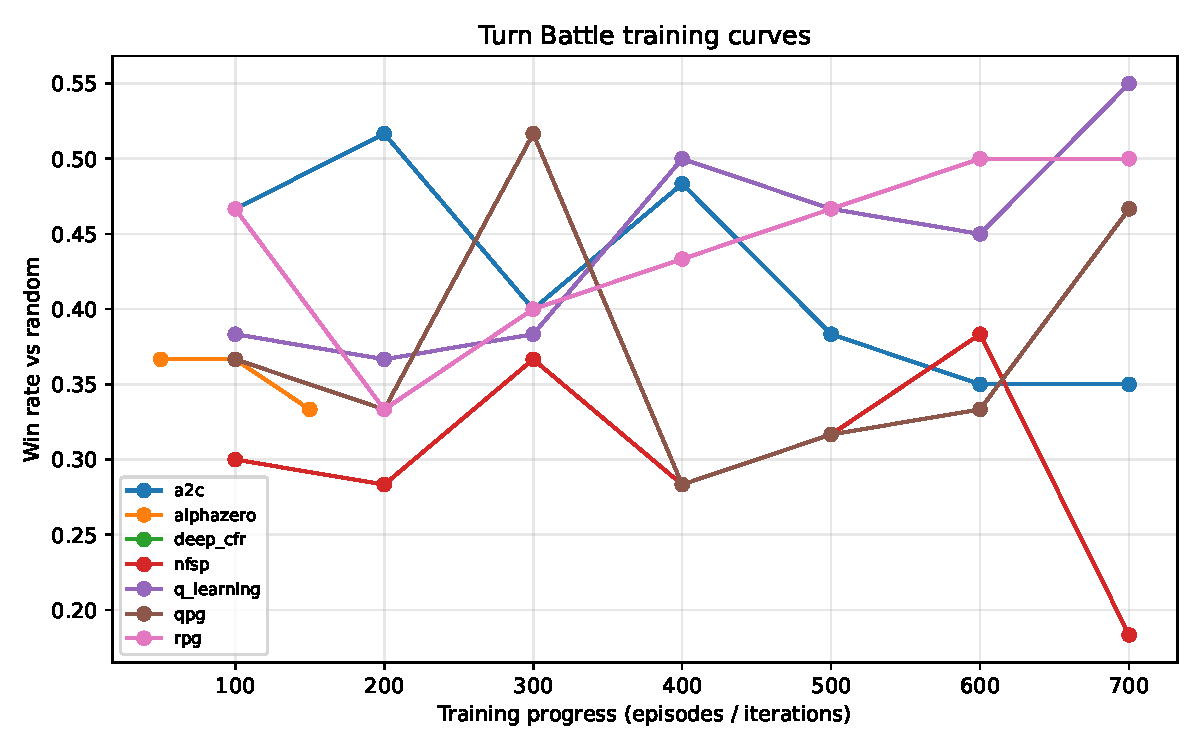
\includegraphics[width=0.9\linewidth]{figures/training_curves.pdf}
\caption{Training progress per algorithm.}
\label{fig:training}
\end{figure}
\section{Seeding}
Algorithms were ranked by win rate vs.\ random before the bracket. MCTS, AlphaZero, and Deep CFR were seeded but excluded from the elimination bracket because they require turn-based evaluation.
\begin{table}[h]
\centering
\begin{tabular}{lc}
\toprule
Algorithm & Win rate vs random \\
\midrule
alphazero & 0.617 \\
qpg & 0.483 \\
deep_cfr & 0.250 \\
nfsp & 0.233 \\
\bottomrule
\end{tabular}
\caption{Seeding scores for all algorithms.}
\end{table}
\begin{figure}[h]
\centering
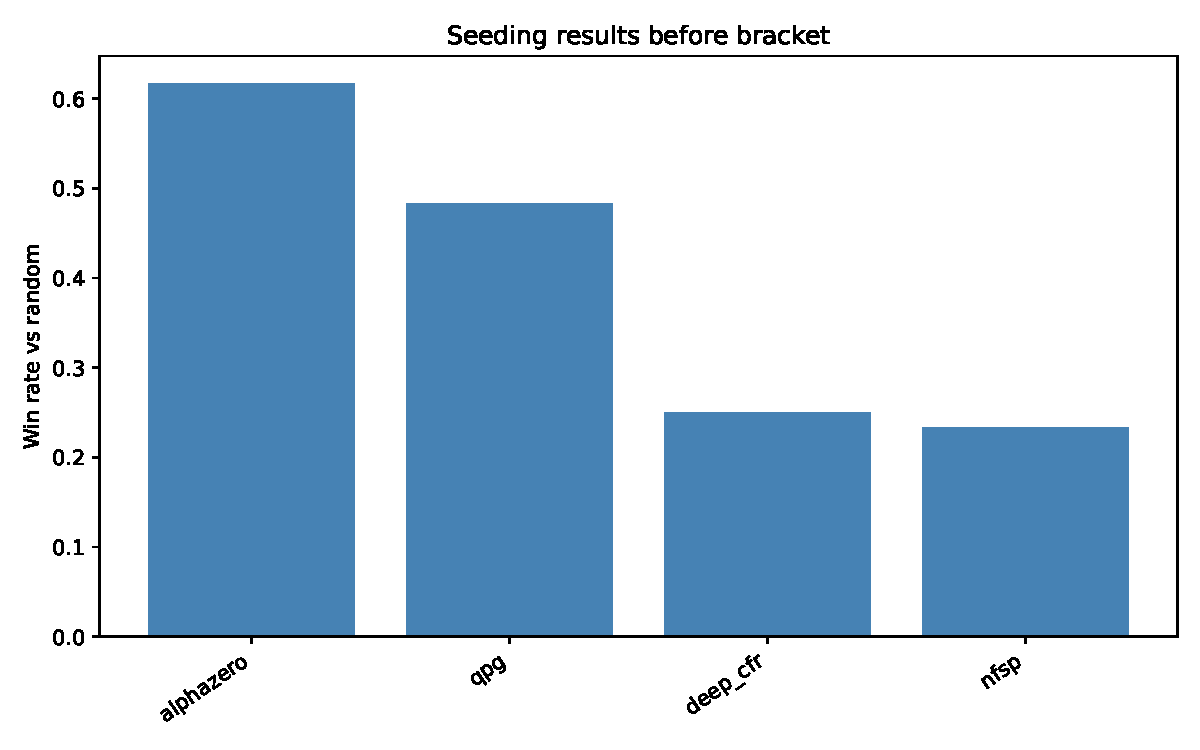
\includegraphics[width=0.9\linewidth]{figures/seeding.pdf}
\caption{Seeding scores.}
\label{fig:seeding}
\end{figure}
\section{Bracket tournament}
The champion was \textbf{alphazero}.
\begin{figure}[h]
\centering
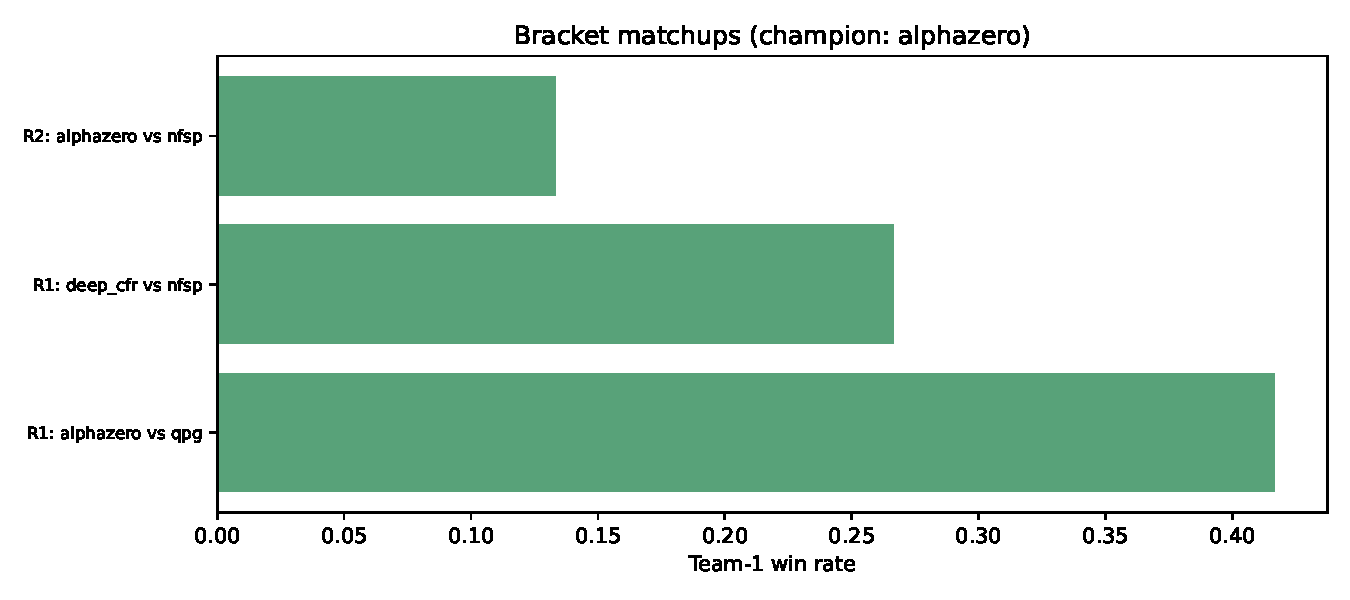
\includegraphics[width=0.95\linewidth]{figures/bracket.pdf}
\caption{Head-to-head bracket results.}
\label{fig:bracket}
\end{figure}
\begin{table}[h]
\centering
\begin{tabular}{llll}
\toprule
Round & Team 1 & Team 2 & Winner \\
\midrule
R1 & alphazero & qpg & alphazero \\
R1 & deep_cfr & nfsp & nfsp \\
R2 & alphazero & nfsp & alphazero \\
\bottomrule
\end{tabular}
\caption{Bracket match log.}
\end{table}
\section{Conclusion}
The bracket winner was \textbf{alphazero}, selected after full training and seeded single-elimination matchups.
\end{document}
